%++++++++++++++++++++++++++++++++++++++++
% Don't modify this section unless you know what you're doing!
\documentclass[letterpaper,11pt]{article}
\usepackage{natbib}
\bibliographystyle{unsrtnat}
\usepackage{tabularx} % extra features for tabular environment
\usepackage{amsmath}  % improve math presentation
\usepackage{graphicx} % takes care of graphic including machinery
\usepackage[margin=1in,letterpaper]{geometry} % decreases margins
%\usepackage{cite} % takes care of citations
\usepackage[final]{hyperref} % adds hyper links inside the generated pdf file
\hypersetup{
	colorlinks=true,       % false: boxed links; true: colored links
	linkcolor=blue,        % color of internal links
	citecolor=blue,        % color of links to bibliography
	filecolor=magenta,     % color of file links
	urlcolor=blue         
}
%+++++++++++++++++++++++++++++++++++++++
\begin{document}

\title{Lab 1E: Joint Comparison \\\textbf{Differntial Drive Robot: Kinematics Modeling}}
\author{ECE183DA/MAE162D}
\date{Due: January 24, 2022}
\maketitle


\section{Lab Overview}
You \textbf{individually} formulate and implement a kinematics model for the Woodbot. You will use the codes and fully implement skeleton codes in the main repository. 

\section{Requirements}
You will individually need to create a forked repository including the following contents: 
\begin{itemize}
    \item A populated git issue tracker, with new issues filed and closed as appropriate
    \begin{itemize}
        \item Tasks assigned to yourself (i.e. determine state representation, write code, etc.)
        \item Tasks assigned to your peers (Use their test\_model.py to validate your KinematicsModel.py)
        \item Tasks assigned to TAs/Profs (For Check off the end-to-end demo)
    \end{itemize}
    \item The symbolic mathematical formulation of the given robot (both dynamics and sensor models) in the docs/ folder
    \item The completed python module sim/robots/KinematicsModel.py implementing the above system models
    \item The completed python module sim/test/test\_model.py ensuring that your KinematicsModel code is correct (and NOPModel is not)
    \item Saved outputs: Graph, video recording, and a corresponding output file for at least one illustrative run
    \item The main Python code that demonstrate your code implementation
\end{itemize}

\subsection{Submission}
Submit a link to the repository on Canvas.
Make sure to assign TAs for check off. We will run your main to test your codes.

Submissions that are late will be accepted with a 50$\%$ grade penalty. 

\section{Methods/Tools}
Each student will be provided the following items:
\begin{itemize}
    \item Python code skeleton
\begin{itemize}
    \item Modular breakdown + API
    \item Input subsystem (Keyboard input, from file, python module, joystick)
    \item Output subsystem (To file, skeleton of to graph on screen, skeleton of 2D animation)
\end{itemize}
    \item Git issues skeleton
\end{itemize}

Go to our repository for more information about how to start coding and what to implement for this lab.
% \href{https://git.uclalemur.com/capstone/lab/kinematics}{https://git.uclalemur.com/capstone/lab/kinematics}.
Link TBD



\appendix

\section{System overview}

\begin{figure}[h!]
  \centering
   \qquad
  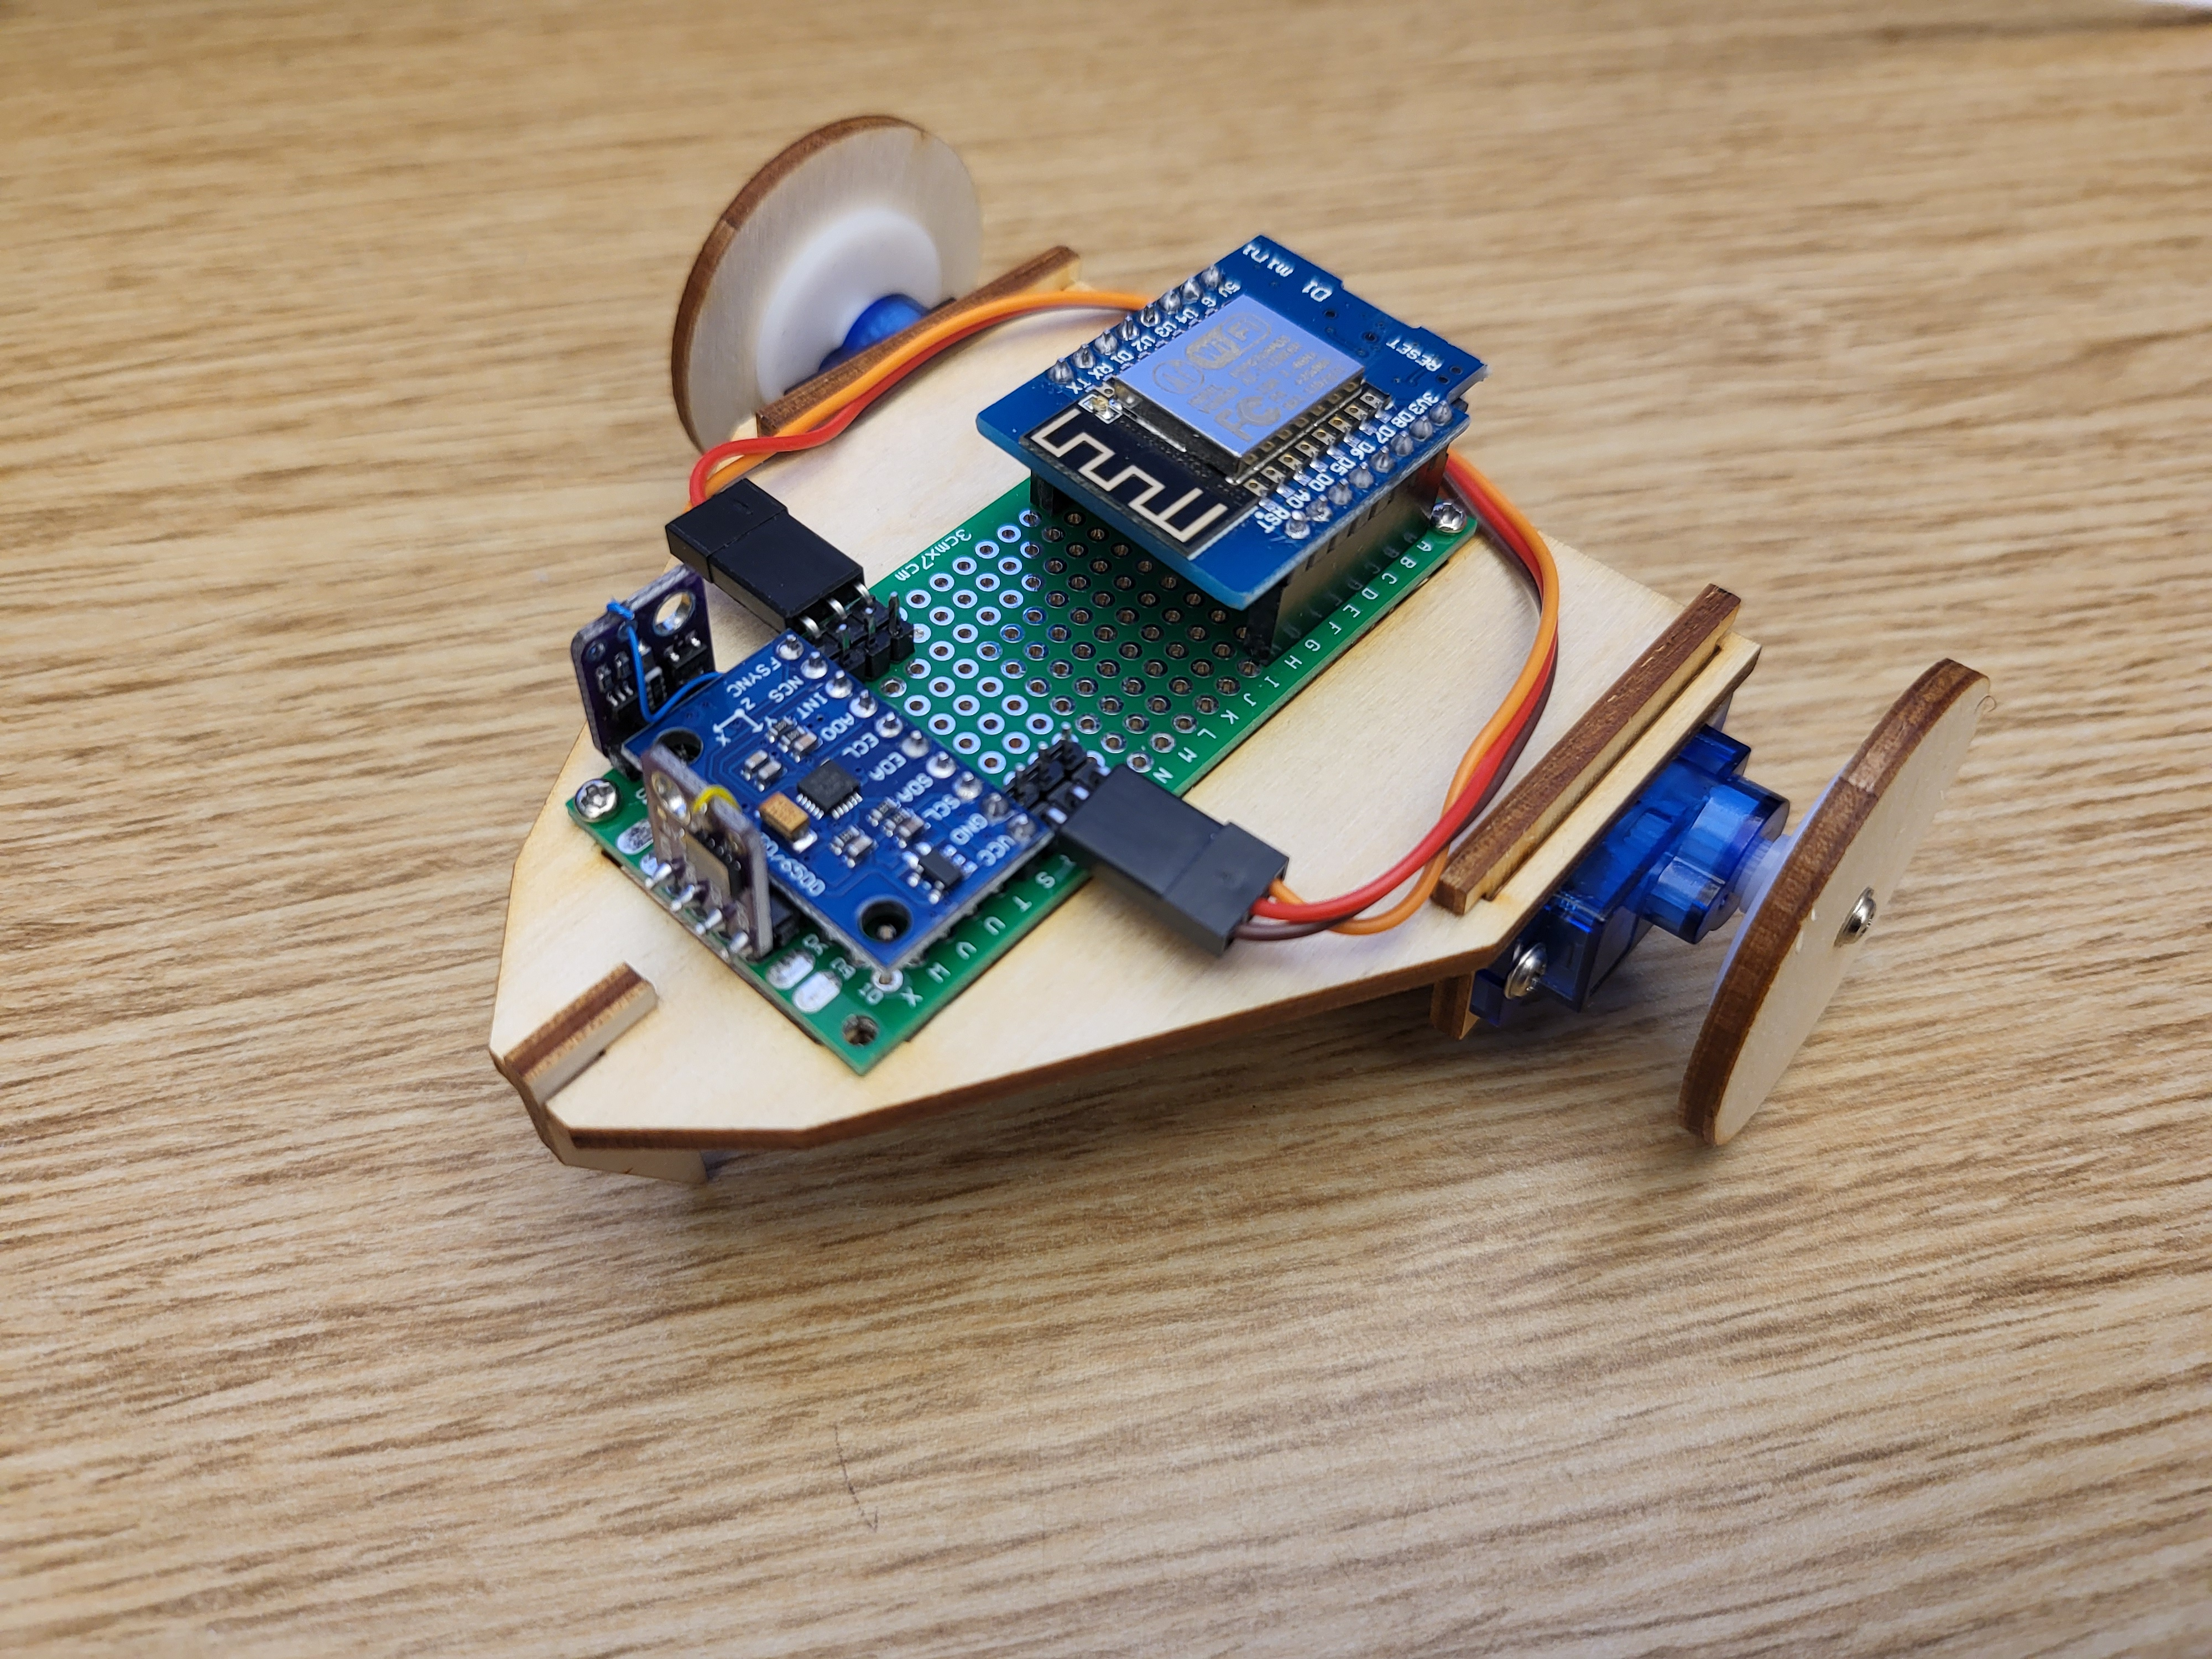
\includegraphics[keepaspectratio,width=\textwidth,height=.15\textheight]{Woodbot.jpg}
  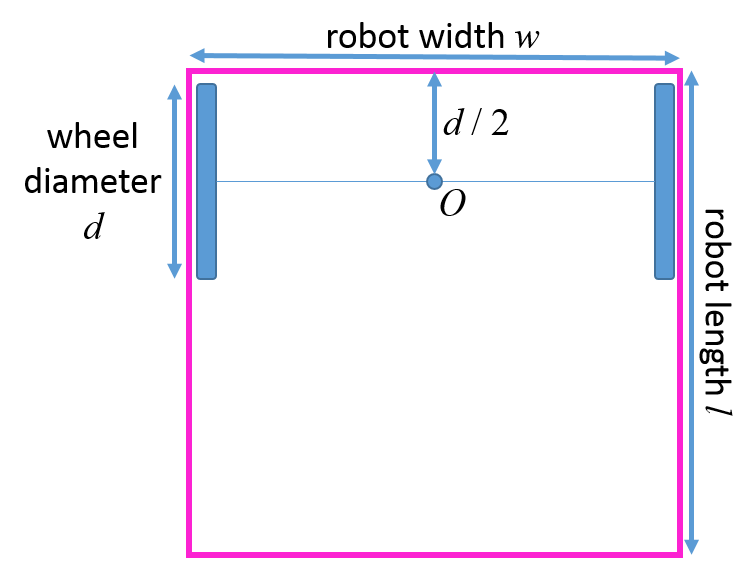
\includegraphics[keepaspectratio,width=\textwidth,height=.15\textheight]{robot}
  \caption{Two wheeled differential drive robots with symbolic dimensions.}
  \label{fg:robot}
\end{figure}

You will model two-wheeled robots similar to the Woodbot shown in Fig.~\ref{fg:robot}. The robot has two wheels of diameter $d = 0.040m 
$, separated by a distance $w \approx 0.1m
$.  Each wheel is direct driven from a continuous rotation servo.  They drag a tail for stability, that contact the ground at a distance $l \approx 0.090m
$ behind their back edge.  The position of each of these robots in the environment is defined relative to their centerpoints $O$. Keep all dimensions symbolic as defined here for the following sections.
%All dimensions should be obtained from the CAD models created by the ME students in section 2.5.1. %dimensions are approximate, and may be different based on manufacturing tolerances.  


We consider two laser range sensors and an IMU for extrinsic position sensing.  The output of these sensors will be a function of the positional state of the robot relative to its environment.
%More details about Paperbot is available at the git repository: \url{https://git.uclalemur.com/mehtank/paperbot}

\subsection{Actuation model}

Each wheel is powered independently by a continuous rotation servo
---part number FS90R---
with the angular velocity of the wheel controlled by a PWM signal from the microcontroller (-1.0 to 1.0).  
The control input to the robot hardware will be the PWM values you send to each wheel, for a total of 2 input variables.  
This allows the robot to drive forwards or backwards at variable speed, or turn with any turning radius.  

%\task{Do we have any other noises in the robot dynamic system?  Explain what they are and how you can add them into the dynamics equations.} %Note that 100\%, 0\% and -100\% correspond to the max speed, 0, and the max in reverse direction, respectively, but again a real motor does not have such linear relationship.


%The mapping from PWM to rotational speed may include nonlinear effects including a deadzone and saturation.  There may also be slippage between the wheels and the floor.
%\task{Use physical experimentation to determine the actuator response and noise models.}

\subsection{Sensing model}

Consider adding two laser range sensors
---part number GYVL53L0X---
and an inertial measurement unit (IMU)
---part MPU9250 IMU--- onto your robot.  %this is the one I use in our lab. it has professional documentation
The output of these sensors will be a function of the state of the robot within its environment.  

The laser range sensors are mounted on the robot such that they measure 1) the distance to a wall in a straight line in front of the robot, and 2) the distance to a wall in a straight line to the right of the robot.  The IMU will return 
1) a measurement of the in-plane rotational speed from a angular rate (gyro) sensor, and 
2) the components of the measured magnetic field along each of the 2 in-plane coordinate axes, which can be used as a compass for absolute orientation relative to Earth's magnetic field.
We will ignore the out-of-plane gyro and magnetometer axes, as well as the accelerometer on the IMU.  Thus this robot will produce 5 output values.



%\task{Use the data sheets for these specific sensors along with physical experimentation to determine their sensor response and noise models.}

\subsection{Environment}
Woodbot runs within a rectangular $1m by 1m$ box.

\subsection{Mathematical formulation}
The state of your robot will satisfy the Markov property, capturing the complete history of actuator inputs to the robot hardware, allowing for computation of the dynamics update as well as all of the sensor measurements.  
\task{Define this state, and then write out the analytic mathematical models for the system dynamics and measurement processes, starting with an ideal theoretical model based on fundamental principles.} 
%Use empirical data from your experiments to quantitatively characterize the noise terms that you have included.

Be sure to clearly define and describe all variables and equations, and produce illustrative diagrams as necessary.  

In the later lab sections we will consider uncertainty of the system. 
%Clearly describe the experiments that were run, the data that was gathered, and the process by which you use that data to mathematically formulate the robotic system.  Include pictures and links to videos.




\end{document}
